\boxde
\BTTN
\begin{ex}%[2D1B3-1]
 Giá trị lớn nhất của hàm số $f(x)=\dfrac{x+1}{x+2}$ trên đoạn $[1;3]$ bằng
 \choice
 {$\dfrac{6}{7}$}
 {$\dfrac{5}{6}$}
 {\True $\dfrac{4}{5}$}
 {$\dfrac{2}{3}$}
 \loigiai{
 Ta có $f'(x)=\dfrac{1}{(x+2)^2}>0\,\forall x\ne 2$.\\
 Do $f(1)=\dfrac{2}{3}$ và $f(3)=\dfrac{4}{5}$, suy ra giá trị lớn nhất của hàm số trên đoạn $[1;3]$ là $\dfrac{4}{5}$.
 }
\end{ex}
\begin{ex}
 \immini{Cho hàm số $y=f(x)$ liên tục trên $[-3;2]$ và có bảng biến thiên như sau. Gọi $M$, $m$ lần lượt là giá trị lớn nhất và giá trị nhỏ nhất của hàm số $y=f(x)$ trên đoạn $[-1;2]$. Giá trị của $M+2m$ bằng
 \choice
 {$6$}
 {$8$}
 {\True $3$}
 {$7$}}{
 
\begin{tikzpicture}
 \tkzTabInit[nocadre=false,lgt=1.2,espcl=1.5,deltacl=0.6]
 {$x$ /.6,$f'(x)$ /.6,$f(x)$ /2}
 {$-3$,$-1$,$0$,$1$,$2$}
 \tkzTabLine{,+,0,-,0,+,0,-,0}
 \tkzTabVar{-/$-2$,+/ $3$ ,-/$0$,+/$2$,-/$1$}
 \end{tikzpicture}}
 \loigiai{
 Từ bảng biến thiên, suy ra $M=3$, $m=0$. Vậy $M+2m=3+2\cdot 0=3$.
 }
\end{ex}
\begin{ex}
 \immini{Cho hàm số $y=f(x)$ có bảng biên thiên như hình bên. Tìm giá trị nhỏ nhất của hàm số trên trên $\mathbb{R}$.
 \choice
 {$2$}
 {$0$}
 {$-3$}
 {\True Không tồn tại}}{
 
\begin{tikzpicture}
 \tkzTabInit[nocadre=false,lgt=1.2,espcl=2.5,deltacl=0.6]
 {$x$ /.6,$f(x)$ /2}
 {$-\infty$,$2$,$+\infty$}
 \tkzTabVar{-/$0$,+/ $2$ ,-/$-3$}
 \end{tikzpicture}}
\end{ex}
\begin{ex}%[2D1B3-1]
 \immini{
 Cho hàm số $ f(x) $ liên tục trên đoạn $ [-1; 3] $ và có đồ thị như hình bên. Gọi $ M $ và $ m $ lần lượt là giá trị lớn nhất và giá trị nhỏ nhất của hàm số trên đoạn $ [-1; 3] $. Giá trị $ M - m $ bằng
 \haicot
 {\True $ 5 $}
 {$ 1 $}
 {$ 4 $}
 {$ 2 $}
 }{
 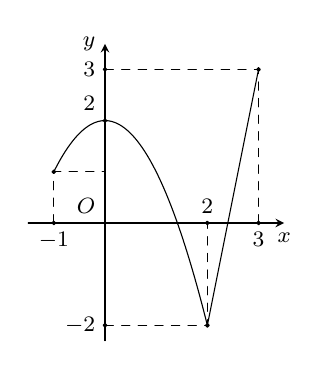
\begin{tikzpicture}[line cap=round,line join=round,x=1.0cm,y=1.0cm,>=stealth,scale=0.65, font = \footnotesize]
 \draw[-> ] (-1.5,0) -- (3.5,0)node[below] {$x$};
 \draw[-> ] (0,-2.3) -- (0,3.5)node[left] {$y$};
 \draw(0,0) node[above left=-0.1] { $O$};
 %	\clip (-.5,-0.5) rectangle (2.3,2.8);
 \draw [samples=100, domain=-1:2] plot (\x, { -( \x )*( \x ) + 2 });
 \draw[fill = black] (0,2) node[above left]{$ 2 $} circle (1pt);
 \draw[fill = black] (0,-2) node[left]{$-2$} circle (1pt);
 \draw[fill = black] (-1,0) node[below]{$-1$} circle (1pt);
 \draw[fill = black] (2,0) node[above]{$2$} circle (1pt);
 \draw[fill = black] (3,0) node[below]{$3$} circle (1pt);
 \draw[fill = black] (0,3) node[left]{$3$} circle (1pt);
 \draw[fill = black] (3,3) circle (1pt);
 \draw[fill = black] (-1,1) circle (1pt);
 \draw[fill = black] (2,-2) circle (1pt);
 \draw (2,-2)--(3,3);
 \draw[dashed] (0,-2)--(2,-2)--(2,0) (-1,0)--(-1,1)--(0,1) (0,3)--(3,3)--(3,0);
 \end{tikzpicture}
 }
 \loigiai{
 Từ hình vẽ, ta thấy $ \heva{&M = 3 \\ & m = - 2} \Rightarrow M - m = 5 $.
 }
\end{ex}
\begin{ex}
 \immini{
 Cho hàm số $y=f(x)$ liên tục trên đoạn $[-3;4]$ và có đồ thị như hình vẽ bên. Gọi $M$ và $m$ lần lượt là các giá trị lớn nhất và nhỏ nhất của hàm số đã cho trên đoạn $[-3;4]$. Tính $M+m$.
 \choice
 {\True $5$}
 {$1$}
 {$8$}
 {$7$}
 }{
 \begin{tikzpicture}[scale=0.6, font=\footnotesize, line join=round, line cap=round, >=stealth]
 \draw [->] (-4,0)--(5,0)node[below]{\footnotesize $x$};
 \draw [->] (0,-1)--(0,6)node[left]{\footnotesize $y$};
 \foreach \y in {5}
 \draw[shift={(0,\y)}](-2pt,0pt) -- (2pt,0pt) node[ left]{\footnotesize $\y$};
 \foreach \y in {3,4}
 \draw[shift={(0,\y)}](-2pt,0pt) -- (2pt,0pt) node[below left]{\footnotesize $\y$};
 \foreach \x in {-3,1,3,4}
 \draw[shift={(\x,0)}](0pt,-2pt) -- (0pt,2pt) node[below]{\footnotesize $\x$};
 \draw [fill=white,draw=black] (0,0) circle (1pt)node[below left] {\footnotesize $O$};
 \draw[smooth,samples=100,domain=0:3] plot(\x,{-(\x)^2+2*(\x)+3});
 \draw (-3,4)--(0,3)
 (3,0)--(4,5);
 \draw[dashed] (-3,0)--(-3,4)--(1,4)--(1,0)
 (4,0)--(4,5)--(0,5);
 \end{tikzpicture}
 }
 \loigiai{
 Dựa vào đồ thị hàm số ta có $\heva{& M=5\\& m=0}\Rightarrow M+m=5$.
 }
\end{ex}
\begin{ex}%[2D1B3-2]
 Cho hàm số $y=f(x)$ có bảng xét dấu đạo hàm như sau:
 \begin{center}
 
\begin{tikzpicture}
 \tikzset{double style/.append style = {draw=\tkzTabDefaultWritingColor,double=\tkzTabDefaultBackgroundColor,double distance=2pt}}
 \tkzTabInit[lgt=1.2,espcl=2,deltacl=0.7]
 {$x$ /.7, $y'$ /.7}
 {$-\infty$,$-1$,$0$,$1$,$+\infty$}
 \tkzTabLine{,-,d,-,$0$,+,$0$,-,}
 \end{tikzpicture}
 \end{center}
 Mệnh đề nào sau đây đúng?
 \choice
 {$\min\limits_{(-1;+\infty)}f(x)=f(0)$}
 {\True $\max\limits_{(0;+\infty)}f(x)=f(1)$}
 {$\max\limits_{(-1;1]}f(x)=f(0)$}
 {$\min\limits_{(-\infty;-1)}f(x)=f(-1)$}
 \loigiai{
 Bổ sung vào bảng biến thiên trên ta có bảng biến thiên như sau:
 \begin{center}
 
\begin{tikzpicture}
 \tkzTabInit
 {$x$ /.7, $f'(x)$ /.7, $f(x)$ /2}
 {$-\infty$,$-1$,$0$,$1$,$+\infty$}
 \tkzTabLine{,-,d,-,$0$,+,$0$,-,}
 \tkzTabVar{+/ ,-D+/ / ,-/$f(0)$,+/$f(1)$,-/ }
 \end{tikzpicture}
 \end{center}
 Từ bảng biến thiên suy ra $\max\limits_{(0;+\infty)}f(x)=f(1)$.
 }
\end{ex}
\begin{ex}
 Giá trị lớn nhất của hàm số $y=-x^2+2x$ bằng
 \choice
 {$5$}
 {\True $1$}
 {$3$}
 {$2$}
 \loigiai{
 Hàm số có đồ thị là một parabol có $a=-1$ nên giá trị lớn nhất của hàm số bằng $y(1)=1$.
 }
\end{ex}
\begin{ex}%[2D1K3]
 Gọi $M$ và $m$ lần lượt là giá trị lớn nhất và giá trị nhỏ nhất của hàm số $y=x^3-3x^2-9x+35$ trên đoạn $\left[ -4;4\right]$. Tính $T=M+2m$.
 \choice
 {$T=-41$}
 {$T=-44$}
 {$T=-43$}
 {\True $T=-42$}
 \loigiai{
 $y'=3x^2-6x-9$\\
 $\hoac{
 &x=-1& &\Rightarrow y=40\\
 &x=3 & &\Rightarrow y=8.}$\\
 Ta có: $y(4)=15$, $y(-4)=-41$.\\
 Suy ra: $M=40$, $m=-41$ nên $T=-42$.}
\end{ex}
\begin{ex}%[2D1B3-3]
 Tìm giá trị nhỏ nhất $m$ của hàm số $f(x)= 4x^2+\dfrac{1}{x}-4$ trên khoảng $(0;+\infty)$.
 \choice
 {\True $m=-1$}
 {$m=-4$}
 {$m=7$}
 {$m=-3$}
 \loigiai
 { Ta có $f(x)=4x^2+\dfrac{1}{x}-4 =4x^2+\dfrac{1}{2x}+\dfrac{1}{2x} -4.$\\
 Áp dụng bất đẳng thức $AM-GM$, ta có $f(x) \geq 3\cdot \sqrt[3]{4x^2 \cdot \dfrac{1}{2x}\cdot \dfrac{1}{2x}} -4 =-1$.
 Đẳng thức xảy ra khi $4x^2=\dfrac{1}{2x} \Leftrightarrow x^3=\dfrac{1}{8} \Leftrightarrow x=\dfrac{1}{2}$.\\
 Vậy $\min\limits_{x\in (0;+\infty)} f(x) =-1$
 }
\end{ex}
\begin{ex}
 Gọi $m$ và $M$ lần lượt là giá trị nhỏ nhất, giá trị lớn nhất của hàm số $y=\dfrac{2x+19}{x^2+16x+68}$. Tính tích $mM$.
 \choice
 {$mM=-0.20$}
 {\True $mM=-0.25$}
 {$mM=-0.15$}
 {$mM=-0.30$}
 \loigiai{
 \begin{itemize}
 \item [$\bullet$] $\mathscr{D} = \mathbb{R}$
 \item [$\bullet$] $y'=\dfrac{-2x^2-38x-168}{(x^2+16x+68)^2}$
 \item [$\bullet$] $y'=0 \Leftrightarrow -2x^2-38x-168=0 \Leftrightarrow x=-7$ hoặc $x=-12$.
 \item [$\bullet$] Bảng biến thiên
 \begin{center}
 
\begin{tikzpicture}
 \tkzTabInit[lgt=1,espcl=3]
 {$x$ /0.7, $y'$ /0.7, $y$ /2}
 {$-\infty$,$-12$,$-7$,$+\infty$}
 \tkzTabLine{,-,$0$,+,$0$,-,}
 \tkzTabVar{+/$0$,-/$-\frac{1}{4}$,+/$1$,-/$0$}
 \end{tikzpicture}
 \end{center}
 Suy ra $m=-\dfrac{1}{4}$, $M=1$. Khi đó $M \cdot m =-\dfrac{1}{4}$.
 \end{itemize}}
\end{ex}
\begin{ex}%[2D1K3-1]%
 Cho hai hàm số $y=f(x)$, $y=g(x)$ có đạo hàm là $f'(x)$, $g'(x)$. Đồ thị hàm số $f'(x)$ và $g'(x)$ được cho như hình vẽ bên dưới.
 \begin{center}
 \begin{tikzpicture}[line join = round, line cap = round,>=stealth,font=\footnotesize,scale=.7]
 \draw[-stealth] (-2.1,0)--(7.5,0) node[below]{$x$};
 \draw[-stealth] (0,-1.6)--(0,4) node[left]{$y$};
 \node[below right] at (0,0) {$O$};
 \coordinate (O) at (0,0);
 \coordinate (A) at (-2,0.5);
 \coordinate (B) at (2,3);
 \coordinate (C) at ($ (7,0.5)$);
 \coordinate (D) at ($ (A)-(0,1.5) $);
 \coordinate (E) at ($ (B) +(0.75,0.5)$);
 \coordinate (H) at (6,1.75);
 \coordinate (F) at ($ (C) +(0,1)$);
 \foreach \x in {-2,-1,1,2,3,4,5,6,7}\draw (\x,0.06)--(\x,-0.06);
 \foreach \y in {-1,1,2,3}\draw (0.06,\y)--(-0.06,\y);
 \draw[thick,teal] (A) .. controls +(5:1.25)
 and +(180:1.15) .. (B) .. controls +(0:1.3)
 and +(170:2.5) .. (C) node[shift={(-0.55,0.5)}]{$ g'(x) $};
 \draw[thick,violet] (D) .. controls +(5:3)
 and +(180:1.25) .. (E) .. controls +(0:0.95)
 and +(160:1.5) .. (H) .. controls +(-20:0.25)
 and +(170:0.25)..(F) node[shift={(-0.55,0.55)}]{$ f'(x) $} ;
 \draw[dashed] (2,0) node[below]{$ 2 $}--(B);
 \draw[dashed] (6,0) node[below]{$ 6 $}--(H);
 \end{tikzpicture}
 \end{center}
 Biết rằng $f(0)-f(6)<g(0)-g(6)$. Giá trị lớn nhất, giá trị nhỏ nhất của hàm số $h(x)=f(x)-g(x)$ trên đoạn $\left[0;6\right]$ lần lượt là
 \choice
 {$h(2)$, $h(6)$}
 {\True$h(6)$, $h(2)$}
 {$h(0)$, $h(2)$}
 {$h(2)$, $h(0)$}
 \loigiai{
 Có $h'(x)=f'(x)-g'(x)$.\\
 Từ đồ thị đã cho ta có bảng biến thiên của hàm số $h(x)$ trên $\left[0;6\right]$
 \begin{center}
 
\begin{tikzpicture}[line join = round, line cap = round,>=stealth,font=\footnotesize,scale=.9]
 \tkzTabInit[espcl=2.5,lgt=1.5]
 {$x$/0.6,$h'(x)$/0.6,$h(x)$/1.8}
 {$0$,$2$,$6$}
 \tkzTabLine{,-,$0$,+,}
 \tkzTabVar{+/$h(0)$,-/$h(2)$,+/$h(6)$}
 \end{tikzpicture}
 \end{center}
 Do đó $\underset{\left[0;6\right]}{\min}\, h(x)=h(2)$.\\
 Giả thiết ta có $f(0)-g(0)<f(6)-g(6)\Leftrightarrow h(0)<h(6)$.\\
 Vậy $\underset{\left[0;6\right]}{\max}\, h(x)=h(6)$.
 }
\end{ex}
\begin{ex}%[2D1K3]
 Giá trị lớn nhất, giá trị nhỏ nhất của hàm số $y=\dfrac{\cos^2x-5\cos x+3}{\cos x-6}$ là
 \choice
 {\True $y_{\max}=\dfrac{1}{5};y_{\min}=-\dfrac{9}{7}$}
 {$y_{\max}=13;y_{\min}=4$}
 {$y_{\max}=1;y_{\min}=-\dfrac{9}{7}$}
 {$y_{\max}=\dfrac{1}{5};y_{\min}=-1$}
 \loigiai{Đặt $t=\cos x, t\in\left[-1;1\right]$, bài toán trở thành tìm giá trị lớn nhất và nhỏ nhất của hàm số $y=\dfrac{t^2-5t+3}{t-6}$ trên đoạn $\left[-1;1\right]$.\\
 Ta có $y'=\dfrac{t^2-12t+27}{(t-6)^2}$; $y'=0\Leftrightarrow \hoac{&t=3\\&t=9}$\\
 Trên đoạn $\left[-1;1\right]$ thì $t^2-12t+27>0\Rightarrow y'>0$ nên hàm số đồng biến. \\
 Vậy giá trị lớn nhất và giá trị nhỏ nhất của hàm số lần lượt là
 $$\underset{}{\mathop{\max}}y=y(1)=\dfrac{1}{5};\underset{}{\mathop{\min}}y=y(-1)=-\dfrac{9}{7}.$$
 }
\end{ex}
\begin{ex}%[2D1B3-1]%
 Cho hàm số $ y=x^3+3 x^2-24 x+2 m $. Có bao nhiêu giá trị nguyên của tham số $ m $ để $\max\limits _{x\in[0; 5]} y\in(0; 10)$.
 \choice
 {$5$}
 {$6$}
 {\True $4$}
 {$9$}
 \loigiai{
 Ta có $ y'=3x^2+6x-24=0\Leftrightarrow\hoac{&x=-4 \, \, \,\mbox{(loại)}\\&x=2 \, \, \,\mbox{(nhận)}.}$ \\
 Ta có bảng biến thiên của hàm số đã cho trên đoạn $ [0; 5] $
 \begin{center}
 
\begin{tikzpicture}
 \tkzTabInit[nocadre=false,lgt=1.2,espcl=2.5,deltacl=0.9]
 {$x $ /0.6, $ y' $ /0.6, $ y $ /2}
 {$0 $, $ 2 $, $ 5$}
 \tkzTabLine{,-, $ 0 $,+,}
 \tkzTabVar{+/ $ 2m $,-/ $-28+2m $,+/ $ 2m+80$}
 \end{tikzpicture}
 \end{center}
 Khi đó $\max\limits _{x\in[0; 5]} y=2m+80\in(0; 10)\Leftrightarrow m\in (-40;-35)$.\\
 Vậy có $ 4 $ giá trị nguyên của tham số $ m $ thỏa bài toán.
 }
\end{ex}
\begin{ex}%[2D1K3-1]
 Cho hàm số $f(x)=(m-1) x^4-2 m x^2+1$ với $m$ là tham số thực. Nếu $\min\limits_{[0; 3]} f(x)=f(2)$ thì $\max\limits_{[0; 3]} f(x)$ bằng
 \choice
 {$-\dfrac{13}{3}$}
 {\True $4$}
 {$-\dfrac{14}{3}$}
 {$1$}
 \loigiai{
 Ta có $f(x)=(m-1) x^4-2 m x^2+1 \Rightarrow f'(x)=4(m-1) x^3-4 m x=4 x\left[(m-1) x^2-m\right]$. \\
 $\Rightarrow f'(x)=0 \Leftrightarrow\left[\begin{aligned}&x=0 \\& (m-1) x^2-m=0.~(*)\end{aligned}\right. $ \\
 Điều kiện cần để $\min\limits_{[0; 3]} f(x)=f(2)$ là phương trình $(*)$ có nghiệm $x=2 \Leftrightarrow 4(m-1)-m=0 \Leftrightarrow m=\dfrac{4}{3}$. \\
 Khi đó $f(x)=\dfrac{1}{3} x^4-\dfrac{8}{3} x^2+1 \Rightarrow f'(x)=\dfrac{4}{3} x^3-\dfrac{16}{3} x$. \\
 $\Rightarrow f'(x)=0 \Leftrightarrow\left[\begin{aligned}&x=0 \in[0; 3] \\& x=2 \in[0; 3] \\& x=-2 \notin[0; 3].\end{aligned}\right. $ \\
 Ta có $f(0)=1; f(3)=4; f(2)=-\dfrac{13}{3}$. \\
 Vậy $\min\limits_{[0; 3]} f(x)=f(2)=-\dfrac{13}{3}$ và $\max\limits_{[0; 3]} f(x)=4$ khi $x=3$.
 }
\end{ex}
\begin{ex}%[2D1K3-6]
 Một loại thuốc được dùng cho một bệnh nhân và nồng độ thuốc trong máu của bệnh nhân được giám sát bởi bác sĩ. Biết rằng nồng độ thuốc trong máu của bệnh nhân sau khi tiêm vào cơ thể trong $ t $ giờ được cho bởi công thức $ c(t)=\dfrac{t}{t^2+1}$(mg/L). Sau khi tiêm thuốc bao lâu thì nồng độ thuốc trong máu của bệnh nhân cao nhất?
 \choice
 {$4 $ giờ}
 {$3 $ giờ}
 {\True $ 1 $ giờ}
 {$2 $ giờ}
 \loigiai{Ta có $ c'(t)=\dfrac{-t^2+1}{\left(t^2+1\right)^{2}},\forall t\in\left(0;+\infty\right)$. Cho $ c'(t)=0\Leftrightarrow\hoac{& t=1\\& t=-1\,\,\text{(loại)}.}$ \\
 Bảng biến thiên
 \begin{center}
 
\begin{tikzpicture}[>=stealth]
 \tkzTabInit[nocadre=false,lgt=1.3,espcl=2,deltacl=0.5]{$t $ /.7, $ c'(t)$ /.7, $ c(t)$ /2}
 {$0 $, $ 1 $, $+\infty$}
 \tkzTabLine{,+, $ 0 $,-,}
 \tkzTabVar{-/,+/,-/}
 \end{tikzpicture}
 \end{center}
 Vậy sau khi tiêm $ 1 $ giờ, nồng độ thuốc trong máu bệnh nhân cao nhất.
 }
\end{ex}
\BTTF
\begin{ex}%[2D1H3-1]
 Hàm số $y=f(x)$ liên tục trên đoạn $[-1;3]$ và có bảng biến thiên như sau.
 \begin{center}
 
\begin{tikzpicture}
 \tkzTabInit[nocadre=false,lgt=1.2,espcl=2]
 {$x$ /0.6,$y'$ /0.6,$y$ /1.7}
 {$-1$,$0$,$2$,$3$}
 \tkzTabLine{,+,$0$,-,$0$,+,}
 \tkzTabVar{-/$0$, +/$5$,-/$1$,+/$4$}
 \end{tikzpicture}
 \end{center}
 Gọi $M$ và $m$ lần lượt là GTLN và GTNN của hàm số trên $[-1;3]$. Xét tính đúng sai của các khẳng định sau:
 \choiceTF
 {$m=f(2)$}
 {$M=f(4)$}
 {\True $m=f(-1)$}
 {\True $M=f(0)$}
 \loigiai{
 Dựa vào bảng biến thiên trên $[-1;3]$, ta có $M=f(0)=5$ và $m=f(-1)=0$.}
\end{ex}
\begin{ex}
 Cho hàm số $y=f(x)$ là hàm liên tục trên $\mathbb{R}$ và có bảng biến thiên như hình vẽ.
 \begin{center}
 
\begin{tikzpicture}
 \tkzTabInit[lgt=1.1,espcl=1.6]{$x$/0.6,$y'$/0.6,$y$/1.7}{$-\infty$,$-1$,$0$,$1$,$+\infty$}
 \tkzTabLine{,+,z,-,z,+,z,-,}
 \tkzTabVar{-/$-\infty$ , +/$4$,-/$3$, +/$4$,-/$-\infty$}
 \end{tikzpicture}
 \end{center}
 Xét tính đúng sai của các khẳng định sau:
 \choiceTF
 {$\min\limits_{(-1;1)}y=3$}
 {\True $\max\limits_{(-1;1)}y=4$}
 {$\min\limits_{\mathbb{R}}y=3$}
 {\True $\max\limits_{\mathbb{R}}y=4$}
 \loigiai{
 \begin{listEX}[1]
 \item [1.] Xét trên $(-1;1)$ thì $\min\limits_{(-1;1)}y=3$ khi $x=0$ và không tồn tại giá trị lớn nhất.
 \item [2.] Xét trên $\mathbb{R}$ thì $\max\limits_{\mathbb{R}}y=4$ khi $x=\pm 1$ và không tồn tại giá trị nhỏ nhất (đừng nhầm lẫn $y=3$ là giá trị nhỏ nhất nhé!)
 \end{listEX}
 }
\end{ex}
\begin{ex}%[2D1H3-2]
 \immini{Cho hàm số $y=f(x)$ liên tục trên $\mathbb{R}$ và có đồ thị như hình bên. Xét tính đúng sai của các khẳng định sau:
 \choiceTF
 {\True Hàm số nghịch biến trên khoảng $(0;1)$}
 {Hàm số đồng biến trên khoảng $(-1;2)$}
 {Hàm số có giá trị lớn nhất bằng $2$}
 {Hàm số có giá trị nhỏ nhất bằng $-1$}
 }{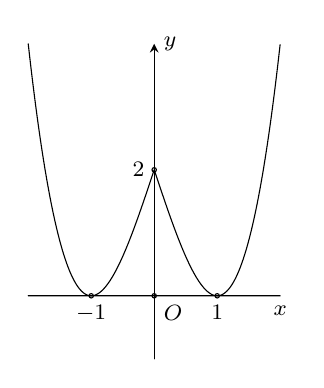
\begin{tikzpicture}[scale=0.8, font=\footnotesize, line join=round, line join=round, line cap = round,>=stealth]
 \draw[->] (-2,0)--(0,0) node[below right]{$O$} circle (1pt)--(2,0) node[below]{$x$};
 \draw[->] (0,-1) --(0,4) node[right]{$y$};
 \foreach \x in {-1,1}{
 \draw (\x,0) node[below]{$\x$} circle (1pt);}
 \foreach \y in {2}{
 \draw (0,\y) node[left]{$\y$} circle (1pt);}
 \draw [domain=0:2, samples=100] %
 plot (\x, {(\x)^3-3*(\x)+2});
 \draw [domain=-2:0, samples=100] %
 plot (\x, {-(\x)^3+3*(\x)+2});
 \end{tikzpicture}
 }
 \loigiai{
 Dựa vào đồ thị hàm số, ta thấy
 \begin{itemchoice}
 \itemch Hàm số nghịch biến trên khoảng $(0;1)$ là khẳng định đúng.
 \itemch Hàm số đồng biến trên khoảng $(-1;2)$ là khẳng định sai.
 \itemch Hàm số có giá trị lớn nhất bằng $2$ là khẳng định sai vì $\lim\limits_{x \to +\infty}f(x)=+\infty$.
 \itemch Hàm số có giá trị nhỏ nhất là $y=0$ (đừng nhầm lẫn với hoành độ nhé!).
 \end{itemchoice}
 }
\end{ex}
\begin{ex}%[2D1K3-6]
 Một người thợ muốn làm một chiếc thùng hình hộp chữ nhật có đáy là hình vuông và không có nắp, biết thể tích của khối hộp là $ V=2{,}16 $ m$ ^3 $. Giá nguyên liệu để làm bốn mặt bên là $ 36000 $ đồng/m$ ^2 $ và giá nguyên liệu để làm đáy là $ 90000 $ đồng/m$ ^2 $. Gọi độ dài cạnh đáy là $ x $ (m) và chiều cao là $ h $ (m).
 \choiceTF
 {Thể tích khối hộp được tính bởi công thức $V=x \cdot h$}
 {Mối liên hệ giữa $x$ và $h$ là $h=\dfrac{2{,}16}{x}$}
 {\True Để chi phí làm chiếc thùng đó thấp nhất thì cạnh đáy là $ 1{,}2 $ m, chiều cao là $ 1{,}8 $ m}
 {\True Số tiền $345\,600$ đồng là chi phí thấp nhất có thể làm chiếc thùng}
 \loigiai{
 \begin{center}
 \begin{tikzpicture}[scale=0.8, font=\footnotesize, line join=round, line cap=round]
 \foreach \x\y\t in {0/0/A,-1/-1.1/B,2.6/-1.1/C}
 \coordinate (\t) at (\x,\y);
 \coordinate (D) at ($(A)+(C)-(B)$);
 \coordinate (A') at ($(A)+(0,3.2)$);
 \coordinate (B') at ($(B)+(0,3.2)$);
 \coordinate (C') at ($(C)+(0,3.2)$);
 \coordinate (D') at ($(D)+(0,3.2)$);
 \draw (B')--(A')--(D')--(C')--(B')--(B)--(C)--(D)--(D')node[midway,right,scale=1]{$h$} (C')--(C);
 \draw[dashed](B)--(A)--(D)node[midway,above,scale=1]{$x$} (A)--(A');
 %\foreach \t/\g in {A/170,B/-150,C/-100,D/0,A'/100,B'/170,C'/-20,D'/50}
 %	\draw[fill=black] (\t) circle(1pt)node[shift={(\g:7pt)}]{$\t$};
 \end{tikzpicture}
 \end{center}
 \begin{itemchoice}
 \itemch Thể tích khối hộp chữ nhật là $V=x \cdot x \cdot h = x^2\cdot h$.
 \itemch Từ $V=x^2\cdot h \Rightarrow h=\dfrac{V}{x^2}=\dfrac{2{,}16}{x^2}$.
 \itemch Diện tích toàn phần của khối hộp $S_{tp}=x^2+4x\cdot h$.\\
 Chi phí làm chiếc thùng là $ f(x)=90x^{2}+4\cdot 36\cdot \dfrac{2{,}16}{x}=90x^{2}+\dfrac{7776}{25x} $. Ta có
 \begin{itemize}
 \item [$\bullet$] $ f'(x)=180x-\dfrac{7776}{25x^{2}}=0\Rightarrow x=1{,}2 $
 \item [$\bullet$] Ta có bảng biến thiên
 \begin{center}
 
\begin{tikzpicture}[>=stealth,scale=1]
 \tkzTabInit[nocadre=false,lgt=1.5,espcl=3]
 {$x$/1,$f'(x)$/1,$f(x)$/1.5}
 {$0$,$1{,}2$,$+\infty$}
 \tkzTabLine{t,-,z,+,}
 \tkzTabVar{+/$+\infty$,-/,+/$+\infty$}
 \end{tikzpicture}
 \end{center}
 Để chi phí làm chiếc thùng nhỏ nhất thì cạnh đáy là $x= 1{,}2 $ m. Suy ra chiều cao là $ h=\dfrac{2{,}16}{1{,}2}=1{,}8 $ m.
 \end{itemize}
 \itemch Khi $x= 1{,}2 $ thì $f(x)=90x^{2}+\dfrac{7776}{25x}=345\,600$ đồng.
 \end{itemchoice}
 }
\end{ex}
\BTTL
\begin{ex}
 Giá trị nhỏ nhất của hàm số $f\left(x\right)=x^3-21x$ trên đoạn $\left[2;19\right]$ bằng bao nhiêu? (làm tròn đến hàng phần chục).\\
 \shortans[3]{$-37$}
 \loigiai{
 Xét trên đoạn $\left[2;19\right]$ hàm số liên tục.\\
 Ta có $f'\left(x\right)=3x^2-21$ . Cho $f'\left(x\right)=0\Rightarrow 3x^2-21=0\Leftrightarrow\hoac{
 x=\sqrt 7\in\left[2;19\right]\\
 x=-\sqrt 7\notin\left[2;19\right].
 }$\\
 Khi đó $f\left(2\right)=-34$ , $f\left(\sqrt 7\right)=-14\sqrt 7 $ , $f\left(19\right)=6460$.\\
 Vậy $\min\limits_{\left[2;19\right]}f\left(x\right)=f\left(\sqrt 7\right)=-14\sqrt 7 \approx -37$ .}
\end{ex}
\begin{ex}
 Tìm giá trị nhỏ nhất của hàm số $y=x^4-2x^2+13$ trên khoảng $(0;+\infty)$.\\
 \shortans[3]{$12$}
 \loigiai{
 Ta có $y'=4x^3-4x$, $y'=0\Leftrightarrow \hoac{& x=1\ \text{(nhận)}\\& x=0\ \text{(loại)}\\& x=-1\ \text{(loại)}.}$\\
 Bảng biến thiên của hàm số trên khoảng $(0;+\infty)$:
 \begin{center}
 
\begin{tikzpicture}
 \tkzTabInit[lgt=1.5,espcl=3,deltacl=0.5]
 {$x$ /.7, $f'(x)$ /.7,$f(x)$ /2}
 {$0$ , $1$ , $+\infty$}
 \tkzTabLine{ ,-,0,+, }
 \tkzTabVar{+/$13$,-/ $12$ ,+/$+\infty$}
 \end{tikzpicture}
 \end{center}
 Dựa vào bảng biến thiên ta có $m=12$.
 }
\end{ex}
\begin{ex}%[MH2017-Lan2-Cau 7]%[2D1B3-1]
 Một vật chuyển động theo quy luật $s=-\dfrac12t^3+9t^2$, với $t$ (giây) là khoảng thời gian tính từ lúc vật bắt đầu chuyển động và $s$ (mét) là quãng đường vật đi được trong khoảng thời gian đó. Hỏi trong khoảng thời gian $10$ giây, kể từ lúc bắt đầu chuyển động, vận tốc (m/s) lớn nhất của vật đạt được bằng bao nhiêu?\\
 \shortans[3]{$54$}
 \loigiai{
 Vận tốc tại thời điểm $t$ là $v(t)=s'(t)=-\dfrac{3}{2}t^2+18t $.\\
 Khi đó yêu cầu bài toán tương đương tìm giá trị lớn nhất của hàm số $y=v(t)=-\dfrac{3}{2}t^2+18t$ trên đoạn $[0;10]$ .\\
 Ta có: $y'=-3t+18=0\Leftrightarrow t=6.$\\
 $y(6)=54;y(0)=0;y(10)=30.$ \\
 Do hàm số $y=v(t)$ liên lục trên đoạn $[0;10]$ nên $\max\limits_{[0;10]}y=54$.
 }
\end{ex}
\begin{ex}%[2D1V3-1]
 Tìm $m$ để hàm số $y=\dfrac{x-m}{mx+1}$ có giá trị nhỏ nhất trên $[0;1]$ bằng $-2$.\\
 \shortans[3]{$2$}
 \loigiai
 {
 Nếu $m=0$ thì hàm số đã cho trở thành $y=x$ có giá trị nhỏ nhất trên $[0;1]$ bằng $0$ (không thỏa mãn yêu cầu bài toán).\\
 Nếu $m \neq 0$ thì hàm số đã cho xác định khi $x\neq -\dfrac{1}{m}$.\\
 Ta có $y'=\dfrac{m^2+1}{(mx+1)^2}>0, \forall x \neq -\dfrac{1}{m}$ nên hàm số đã cho luôn đồng biến trên mỗi khoảng xác định của nó.\\
 Hàm số đã cho có giá trị nhỏ nhất trên $[0;1]$ bằng $-2$ khi
 \[\heva{&\hoac{&-\dfrac{1}{m}<0 \\&-\dfrac{1}{m}>1} \\&y(0)=-2} \Leftrightarrow \heva{&\hoac{&m>0 \\&-1<m<0} \\&-m=-2} \Leftrightarrow m=2.\]
 }
\end{ex}
\begin{ex}%[2D1T3-6]
 Mỗi đợt xuất khẩu gạo của tỉnh A thường kéo dài trong $60$ ngày. Người ta nhận thấy lượng gạo xuất khẩu tính theo ngày thứ $t$ được xác định bởi công thức: $S(t)=\dfrac{2}{5}t^3-63t^2+3240t-3100$ (tấn) $(1 \le t \le 60)$. Hỏi trong $60$ ngày đó, ngày thứ mấy có lượng gạo xuất khẩu cao nhất?\\
 \shortans[3]{$45$}
 \loigiai{Xét hàm số $S(t)=\dfrac{2}{5}t^3-63t^2+3240t-3100$ với $t \in [1;60]$.\\
 Ta có $S'(t)=\dfrac{6}{5}t^2-126t+3240$.\\
 \hspace*{1cm} $S'(t)=0 \Leftrightarrow \hoac{&t=45 \\ &t=60.}$\\
 Vì $S(1)=\dfrac{387}{5}, S(45)=51575, S(60)=50900$ nên ta được $\max \limits_{t \in [1;60]} S(t)=S(45)=51575$.\\
 Vậy ngày thứ $45$ là ngày có lượng gạo xuất khẩu cao nhất.}
\end{ex}
\begin{ex}%[2D1C3-6]
 Một xưởng in có $8$ máy in, mỗi máy in được $3\;600$ bản in trong một giờ. Chi phí để vận hành một máy in trong mỗi lần in là $50$ nghìn đồng. Chi phí cho $n$ máy in chạy trong một giờ là $60(6n+10)$ nghìn đồng. Hỏi nếu in $50\;000$ tờ quảng cáo thì phải sử dụng bao nhiêu máy in để được lãi nhiều nhất?	\\
 \shortans[3]{$5$}
 \loigiai
 {Một máy trong một giờ in được $3\;600$ tờ nên $50\;000$ tờ cần $\dfrac{125}{9}$ giờ.\\
 Do đó $n$ máy cần thời gian là $\dfrac{125}{9n}$ giờ.\\
 Tổng chi phí là $f(n)=\left[10\cdot \left(6n+10\right)\right]\cdot 1\,000+50\;000n$.\\
 Khi đó, để lãi nhiều nhất thì $f(n)$ đạt giá trị nhỏ nhất, với $n\in \left[1;8\right]$ và $n\in \mathbb{N}$.\\
 Cách 1: Khảo sát hàm số $f(n)$ trên miền $[1;8]$.\\
 Cách 2: $f(n)=\left(\dfrac{250}{3}+\dfrac{1250}{9n}+5n\right)\cdot 10\,000\geq \left(\dfrac{250}{3}+\dfrac{50\sqrt{10}}{3}\right)$ (BĐT AM - GM).\\
 Do đó, $f(n)$ nhỏ nhất khi $\dfrac{1\,250}{9n}=4n\Leftrightarrow n =\dfrac{5\sqrt{5}}{10}\approx 5$.\\
 Cách 3: Dùng Table lập bảng $f(n)$ với $n\in \left\{1; 2; \ldots ; 8\right\}$ từ đó suy ra $n=5$.
 }
\end{ex}